\documentclass{article}
\usepackage{fontspec}
\setmainfont{Times New Roman}
\usepackage{geometry}
\usepackage{CTEX}
\geometry{papersize={21cm,29.7cm}}
\geometry{left=3.18cm,right=3.18cm,top=2.54cm,bottom=2.54cm}
\usepackage{fancyhdr}
\usepackage{amsmath}
\pagestyle{fancy}
\lhead{学号:202000460020}
\rhead{姓名:苏博南}
\cfoot{\thepage}
\renewcommand{\headrulewidth}{0.4pt}
\renewcommand{\headwidth}{\textwidth}
\usepackage{tikz}
\usetikzlibrary{automata, positioning, arrows}
\usepackage{listings}

\newtheorem{question}{题目}  
\lstset{
	basicstyle=\small\ttfamily,	% 基本样式
		keywordstyle=\color{blue}, % 关键词样式
		commentstyle=\color{gray!50!black!50},   	% 注释样式
		stringstyle=\rmfamily\slshape\color{red}, 	% 字符串样式
	backgroundcolor=\color{gray!0},     % 代码块背景颜色
	frame=leftline,						% 代码框形状
	framerule=12pt,%
		rulecolor=\color{gray!0},      % 代码框颜色
	numbers=left,				% 左侧显示行号往左靠, 还可以为right ,或none,即不加行号
		numberstyle=\footnotesize\itshape,	% 行号的样式
		firstnumber=1,
		stepnumber=1,                  	% 若设置为2,则显示行号为1,3,5
		numbersep=7pt,               	% 行号与代码之间的间距
	aboveskip=.25em, 			% 代码块边框
	showspaces=false,               	% 显示添加特定下划线的空格
	showstringspaces=false,         	% 不显示代码字符串中间的空格标记
	keepspaces=true, 					
	showtabs=false,                 	% 在字符串中显示制表符
	tabsize=2,                     		% 默认缩进2个字符
	captionpos=b,                   	% 将标题位置设置为底部
	flexiblecolumns=true, 			%
	breaklines=true,                	% 设置自动断行
	breakatwhitespace=false,        	% 设置自动中断是否只发生在空格处
	breakautoindent=true,			%
	breakindent=1em, 			%
	title=\lstname,				%
	escapeinside=``,  			% 在``里显示中文
	xleftmargin=1em,  xrightmargin=1em,     % 设定listing左右的空白
	aboveskip=1ex, belowskip=1ex,
	framextopmargin=1pt, framexbottommargin=1pt,
        abovecaptionskip=-2pt,belowcaptionskip=3pt,
	% 设定中文冲突,断行,列模式,数学环境输入,listing数字的样式
	extendedchars=false, columns=flexible, mathescape=true,
	texcl=true,
	fontadjust
}%

\begin{document}

\begin{center}
    \huge{机器学习课程实验五}\\
    \large{\today \quad 苏博南\quad 202000460020}
\end{center}

\section{Regularize Linear Regression}

考虑解决overfitting的问题,将parameter引入Cost Function:
\begin{equation}
    \begin{split}
        J(\theta)=\frac{1}{2m}[\sum_{i=1}^m(h_\theta(x^{(i)})-y^{(i)})^2+\lambda\sum_{j=1}^n\theta_j^2]
    \end{split} 
\end{equation}
通过$\nabla J(\theta)=0$可以解得:
\begin{equation}
    \begin{split}
        \theta^*=(X^TX+\lambda\begin{pmatrix}0 & & & \\ & 1 & & \\ & & \ddots & \\ & & & 1\end{pmatrix})^{-1}X^Ty
    \end{split}
\end{equation}
分别取$\lambda=0,\lambda=1,\lambda=10$可以做的如图1所示预测结果:
\begin{figure}[h]
    \centering
    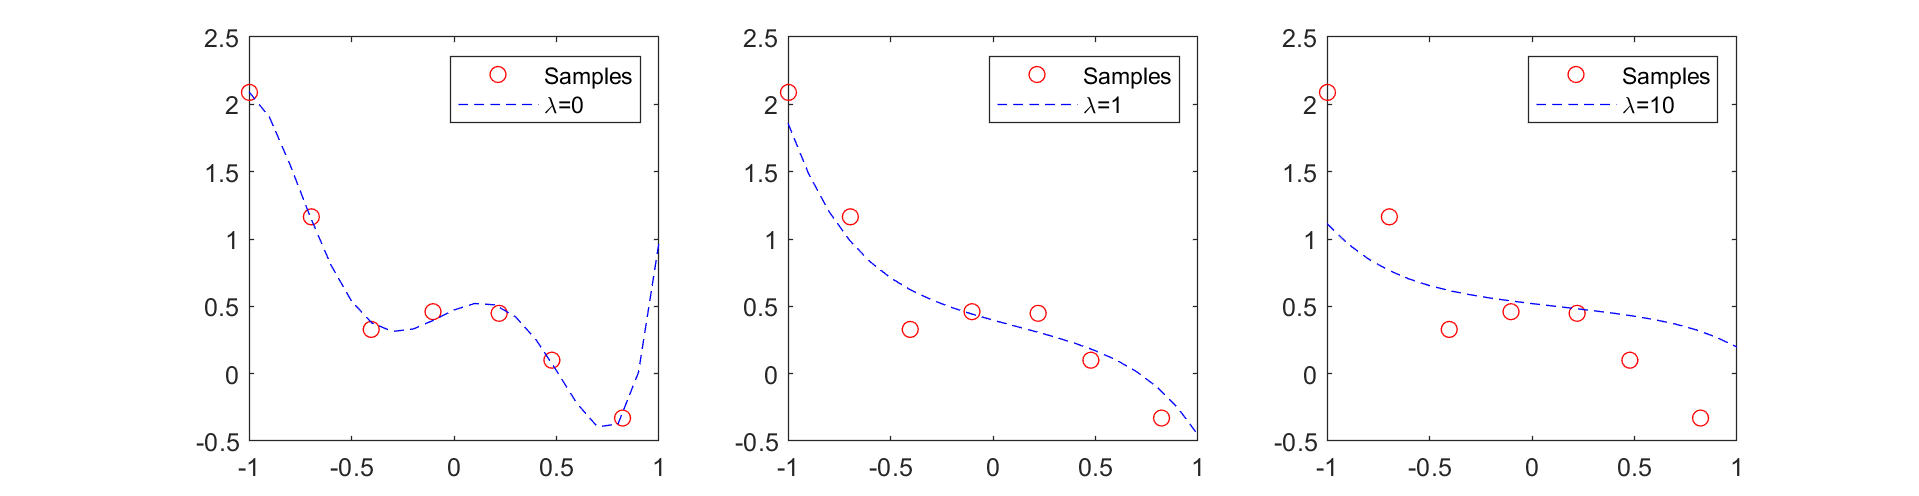
\includegraphics[width=\linewidth]{1.png}
    \caption{拟合结果}
\end{figure}

代码:
\begin{lstlisting}
    x = load('ex5Data/ex5Linx.dat');
    y = load('ex5Data/ex5Liny.dat');


    [m, n] = size(x);
    X = [ones(m, 1), x, x.^2, x.^3, x.^4, x.^5];
    [m, n] = size(X);
    reg = diag([0, ones(1, n - 1)]);
    xs = [-1 : 0.1 : 1]';

    subplot(1, 3, 1);
    plot(x, y, 'rO');
    hold on;
    lambda = 0;
    theta = inv(X' * X + lambda * reg) * X' * y;
    ys = [ones(21, 1), xs, xs.^2, xs.^3, xs.^4, xs.^5] * theta;
    plot(xs, ys, 'b--');
    legend('Samples', '\lambda=0');

    subplot(1, 3, 2);
    plot(x, y, 'rO');
    hold on;
    lambda = 1;
    theta = inv(X' * X + lambda * reg) * X' * y;
    ys = [ones(21, 1), xs, xs.^2, xs.^3, xs.^4, xs.^5] * theta;
    plot(xs, ys, 'b--');
    legend('Samples', '\lambda=1');

    subplot(1, 3, 3);
    plot(x, y, 'rO');
    hold on;
    lambda = 10;
    theta = inv(X' * X + lambda * reg) * X' * y;
    ys = [ones(21, 1), xs, xs.^2, xs.^3, xs.^4, xs.^5] * theta;
    plot(xs, ys, 'b--');
    legend('Samples', '\lambda=10');

\end{lstlisting}

\section{Regularize Logistic Regression}

在预处理完数据后,类似Linear Regression,可以将parameters引入Cost Function:
\begin{equation}
    \begin{split}
        J(\theta)=-\frac{1}{m}[y^{(i)}ln(h_\theta(x^{(i)}))+(1-y^{(i)})ln(1-h_\theta(x^{(i)}))]+\frac{\lambda}{2m}\sum_{j=1}^n\theta_j^2
    \end{split}
\end{equation}

利用牛顿法迭代:
\begin{equation}
    \begin{split}
        \theta^{(t+1)}=\theta^{(t)}-H^{-1}\nabla_\theta J
    \end{split}
\end{equation}
其中,
\begin{equation}
    \begin{split}
        \nabla_\theta J=\begin{pmatrix}
            \frac{1}{m}\sum_{i=1}^m(h_\theta(x^{(i)})-y^{(i)})x_0^{(i)} \\
            \frac{1}{m}\sum_{i=1}^m(h_\theta(x^{(i)})-y^{(i)})x_1^{(i)} +\frac{\lambda}{m}\theta_1\\
            \frac{1}{m}\sum_{i=1}^m(h_\theta(x^{(i)})-y^{(i)})x_2^{(i)} +\frac{\lambda}{m}\theta_2\\
            ......\\
            \frac{1}{m}\sum_{i=1}^m(h_\theta(x^{(i)})-y^{(i)})x_n^{(i)} +\frac{\lambda}{m}\theta_n\\
        \end{pmatrix}\\
        H=\frac{1}{m}[\sum_{i=1}^mh_\theta(x^{(i)})(1-h_\theta(x^{(i)}))x^{(i)}(x^{(i)})^T]+\frac{\lambda}{m}\begin{pmatrix}
            0& & & \\ & 1 & & \\ & & \ddots & \\ & & & 1 
        \end{pmatrix}
    \end{split}
\end{equation}
代码如下:



\begin{lstlisting}
    x = load('ex5Data/ex5Logx.dat');
    y = load('ex5Data/ex5Logy.dat');

    pos = find(y); 
    neg = find(y == 0);


    X = map_feature(x(:, 1), x(:, 2));
    [m, n] = size(X);
    plot(x(pos, 1), x(pos, 2), '+');
    hold on;
    plot(x(neg, 1), x(neg, 2), 'o');
    % lambda = 1;
    % lambda = 0;
    lambda = 1;
    theta = zeros(n, 1);
    for it = 1 : 10
        grad = X' * (sigmond(X * theta) - y) / m;
        reg = lambda / m .* theta;
        reg(1) = 0;
        grad = grad + reg;
        H = X' * diag(sigmond(X * theta) .* sigmond(-X * theta), 0) * X / m + lambda / m .* diag([0, ones(1, n - 1)]);
        theta = theta - H \ grad;
    end

    u = linspace(-1, 1.5, 200);
    v = linspace(-1, 1.5, 200);
    z = zeros(length(u), length(v));

    for i = 1 : length(u)
        for j = 1 : length(v)
            z(j, i) = map_feature(u(i), v(j)) * theta;
        end
    end
    contour(u, v, z, [0, 0], 'LineWidth', 2);
    legend('y=1', 'y=0', 'decision bound');
\end{lstlisting}

然后作出$P(y=1\;|\;x;\theta)=0.5$的图像,即$\theta^Tx=0$:
\begin{figure}[h]
    \centering
    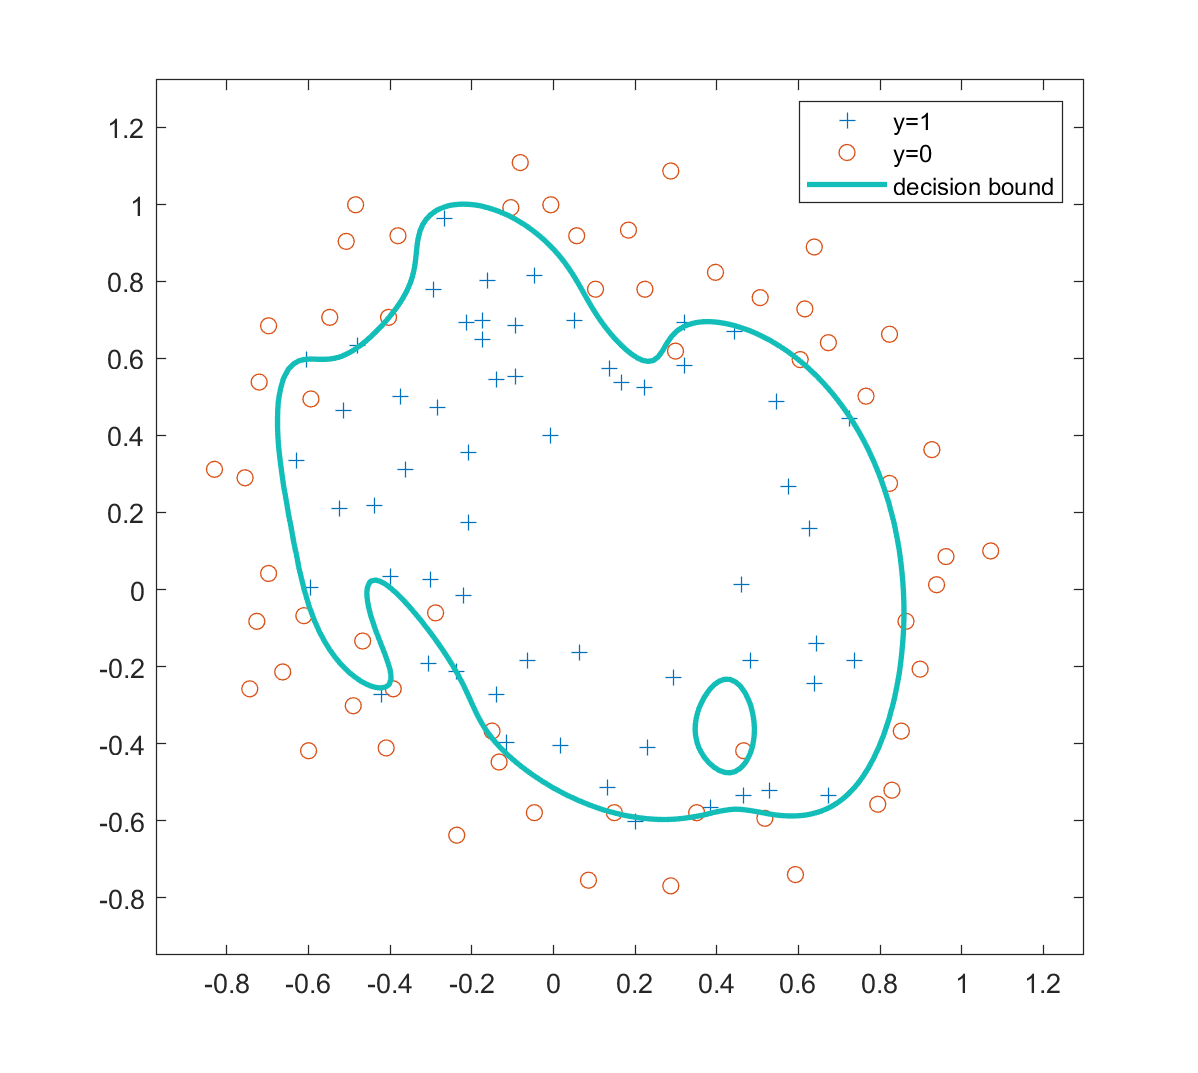
\includegraphics[width=0.5\linewidth]{lambda=0.png}
    \caption{$\lambda=0$}
\end{figure}
\begin{figure}[h]
    \centering
    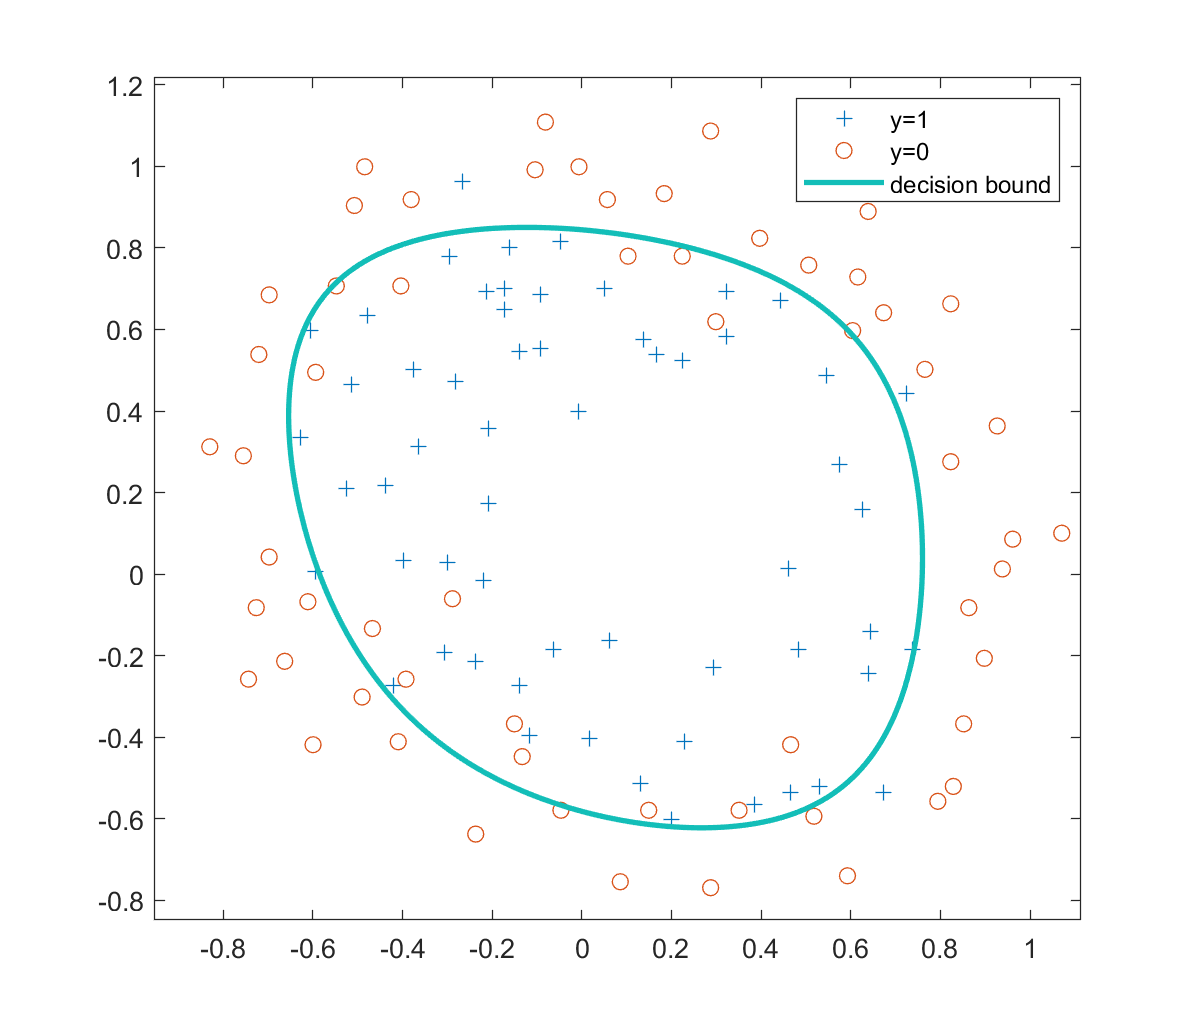
\includegraphics[width=0.5\linewidth]{lambda=1.png}
    \caption{$\lambda=1$}
\end{figure}
\begin{figure}[h]
    \centering
    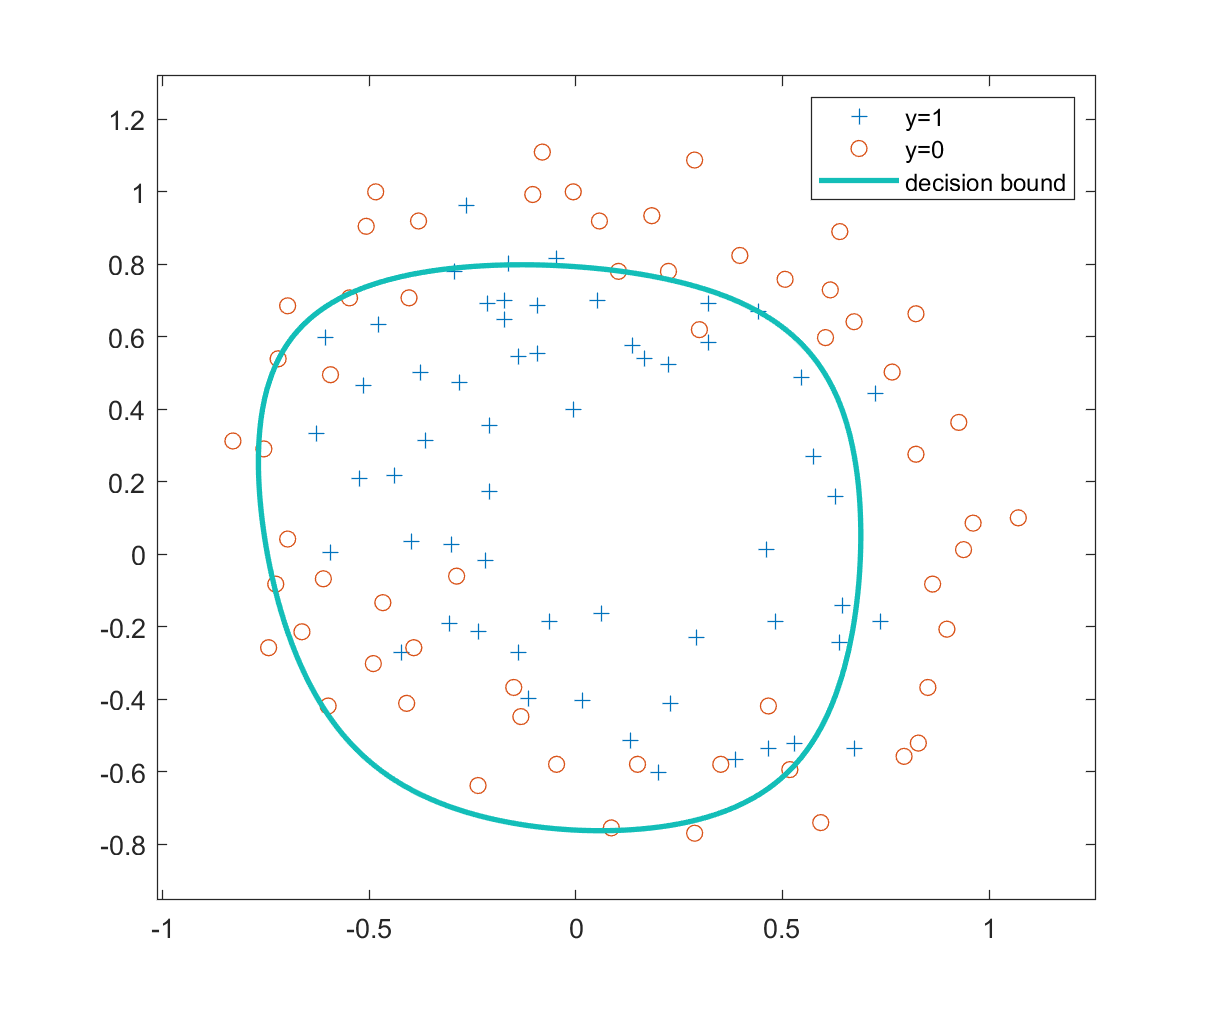
\includegraphics[width=0.5\linewidth]{lambda=10.png}
    \caption{$\lambda=10$}
\end{figure}




可以看到,当$\lambda$越大,分界线越平滑和规则,更接近一个规则图形,不规则的边界减少。

\end{document}